\pagebreak
\'Etudier une fonction c'est déterminer tous les éléments (tangentes, asymptotes) qui permettent d'obtenir l'allure de la courbe représentative de la fonction.\\

\begin{exm}
	\[
		f: x \mapsto  \frac{x^2-2x+3}{x^2+2x-3}
	\] 
	\begin{enumerate}
		\item On détemine le domaine de définition de la fonction $f$.\\
			Soit $x \in \R$. \[
				x^2+2x-3 = 0 \iff x \in \{-3,1\} \quad \text{ car }
				\begin{cases}
					-3 + 1 = -2 = -\frac{b}{a}\\
					-3 \times 1 = -3 = \frac{c}{a}
				\end{cases}
			\] Donc $f$ est définie sur $\mathcal{D}$ avec $\mathcal{D} = ]-\infty, -3[ \cup ]-3,-1[ \cup ]-1, +\infty[$
		\item Asymptotes et limites\\
			Soit $x \in \mathcal{D}$\\
			\[
				f(x) = \frac{\cancel{x^2}\left( 1-\frac{2}{x}+\frac{3}{x^2} \right)}{\cancel{x^2}\left( 1+\frac{2}{x}-\frac{3}{x^2} \right) }
				\tendsto{x\to \pm \infty} 1
			\] 
			\[
				\begin{rcases*}
					x^2-2x + 3 \tendsto{x\to -3} 9+6+3 = 18\\
					x^2+ 2x - 3 \tendsto{x\to -3} 0
				\end{rcases*} \text{ donc }
				\begin{cases}
					f(x) \tendsto{\substack{x \to -3\\<}} +\infty\\
					f(x) \tendsto{\substack{x \to -3\\>}} -\infty\\
				\end{cases}
			\]\[
				\begin{rcases*}
					x^2-2x + 3 \tendsto{x\to 1} 2\\
					x^2+ 2x - 3 \tendsto{x\to 1} 0
				\end{rcases*} \text{ donc }
				\begin{cases}
					f(x) \tendsto{\substack{x \to 1\\<}} -\infty\\
					f(x) \tendsto{\substack{x \to 1\\>}} +\infty\\
				\end{cases}
			\] 
		\item $f$ est dérivable sur $\mathcal{D}$ et 
			\begin{align*}
				\forall x \in \mathcal{D}, f'(x) &= \frac{2(x-1)(x^2+2x-3) - 2(x^2-2x+3)(x+1)}{(x^2+2x-3)^2}\\
				&= \frac{2(2x^2 - 6x)}{(x^2-2x+3)^2} \\
				&= \frac{4x(x-4)}{(x^2-2x+3)^2} \\
			\end{align*}
			\begin{center}
				\begin{tikzpicture}
					\tkzTabInit[espcl=1.5]{$x$/0.7,$f'(x)$/1,$f$/2}{$+\infty$, -3, 0, 1, 3, +$\infty$}
					\tkzTabLine{,+,d,+,z,-,d,-,z,+,}
					\tkzTabVar{-/1,+D-/$+\infty$/$-\infty$, +/-1, -D+/$-\infty$/$+\infty$, -/$\frac{1}{2}$, +/1}
				\end{tikzpicture}
			\end{center}

			\begin{center}
				\begin{asy}
					import graph;
					import math;

					size(10cm);
					xaxis(LeftTicks, EndArrow);
					yaxis(EndArrow);

					labely(-2); ytick(-2);
					labely(2); ytick(2);
					ytick(0);

					real f(real x) {return (x^2-2x+3)/(x^2+2x-3);}

					bool3 fcond(real x) {
						if(x == -3 || x == 1 || abs(f(x)) > 3)
							return false;
						else
							return true;
					}

					draw(graph(f, -10, 10, n=10*ngraph, cond=fcond));

					drawline((0,1),(1,1), dashed+green);

					real eps = 1;

					void drawtangent(real x) {real y = f(x); draw((x-eps, y) -- (x + eps, y),red, Arrows(TeXHead)); }

					drawtangent(0);
					drawtangent(3);

					crop();
				\end{asy}
			\end{center}
	\end{enumerate}
\end{exm}
